% METODOLOGIA

\chapter{METODOLOGIA}
\label{chap:metodologia}

Este capítulo descreve os procedimentos metodológicos adotados para investigar o impacto do uso do ChatGPT no desempenho dos estudantes em Algoritmos e Estruturas de Dados, com foco em Heap e Tabelas Hash. O estudo adota um desenho experimental com grupos cruzados, no qual as condições de uso da ferramenta são invertidas entre os dois tópicos investigados.

\section{Caracterização da Pesquisa}
\label{sec:caracterizacao-pesquisa}

A pesquisa caracteriza-se como um estudo empírico em contexto educacional, com abordagem quantitativa e desenho comparativo. O objetivo é observar se o uso do ChatGPT em atividades práticas de programação influencia o desempenho dos estudantes nos conteúdos trabalhados. Para isso, adota-se um desenho experimental com dois grupos e condições invertidas de uso da ferramenta entre os tópicos Heap e Tabelas Hash \cite{wohlin2012experimentation}.

Neste estudo, o \textbf{desempenho} é operacionalizado como a pontuação obtida por cada estudante em questionários objetivos de múltipla escolha, aplicados ao final de cada atividade prática, sem apoio do ChatGPT. O questionário de Heap continha 20 questões e o de Tabelas Hash, 21. A pontuação corresponde ao número de acertos, com o mesmo peso por questão, resultando em escalas de 0 a 20 e de 0 a 21, respectivamente. Essa medida permite comparar o desempenho nas condições com e sem uso da ferramenta durante as implementações.

\section{Contexto e Participantes}
\label{sec:contexto-participantes}

O estudo foi conduzido na disciplina de Algoritmos e Estruturas de Dados, vinculada ao curso de Engenharia da Computação da Universidade Federal Rural de Pernambuco, na Unidade Acadêmica de Belo Jardim, no primeiro semestre letivo de 2026 (2026.1). A disciplina integra tipicamente o terceiro período da grade curricular e tem, como formação prévia esperada, conteúdos de Programação Orientada a Objetos (ou equivalente). O experimento ocorreu no final da disciplina. As atividades práticas foram implementadas em Java, linguagem adotada no componente curricular.

Os participantes foram estudantes regularmente matriculados no período de aplicação do estudo. A participação foi voluntária, precedida da apresentação dos objetivos da pesquisa e do aceite por meio do termo de consentimento livre e esclarecido (TCLE). Como incentivo acadêmico, a participação nas atividades experimentais valeu 1 ponto na disciplina. Os dados analisados foram tratados de forma agregada ou anonimizada, preservando a confidencialidade dos participantes. Ao todo, 28 estudantes responderam ao formulário inicial vinculado ao TCLE; desses, 25 integraram a distribuição experimental nos grupos --- três estudantes que responderam ao formulário não compareceram no dia da alocação aos grupos e, portanto, não participaram das atividades experimentais.

\section{Conteúdos Investigados}
\label{sec:conteudos-investigados}

Este TCC concentra-se nos conteúdos de Heap e Tabelas Hash, escolhidos por combinarem fundamentos conceituais, análise de complexidade e desafios de implementação relevantes na formação em Computação \cite{cormen2022introduction}. Heap foi o primeiro conteúdo trabalhado no experimento; Tabelas Hash, o segundo, com inversão das condições de uso do ChatGPT entre os grupos.

\section{Hipótese da Pesquisa}
\label{sec:hipotese-pesquisa}

A investigação considera uma única hipótese nula, associada ao desempenho nos questionários após as atividades práticas:

\begin{itemize}
    \item $H_{0}$: não há diferença significativa no desempenho dos estudantes --- medido pela pontuação nos questionários --- quando comparamos condições com e sem uso do ChatGPT nas atividades práticas de Algoritmos e Estruturas de Dados.
\end{itemize}

A hipótese $H_{0}$ é avaliada por meio das pontuações obtidas nos questionários aplicados após cada atividade prática, comparando o desempenho dos estudantes em Heap e Tabelas Hash sob cada condição experimental. A análise estatística considera o tamanho da amostra e a distribuição dos dados, empregando testes não paramétricos quando necessário \cite{kitchenham2019statistical,sheskin2003handbook}.

\section{Desenho Experimental}
\label{sec:desenho-experimental}

O desenho experimental é organizado em três momentos principais: etapa inicial, atividade de Heap e atividade de Tabelas Hash. Em cada atividade prática, a avaliação do desempenho foi realizada por meio de um questionário aplicado ao final da implementação, sem uso do ChatGPT. A Figura \ref{fig:fluxo-metodologia} apresenta uma visão geral do processo. Nela, a etapa experimental inicia com 25 estudantes distribuídos nos grupos; a análise comparativa final considera apenas os 20 participantes com participação completa, isto é, que cumpriram todas as etapas da pesquisa --- do formulário de perfil até o último questionário.

\begin{figure}[!ht]
    \SingleSpacing
    \centering
    \caption{Visão geral do processo experimental.}
    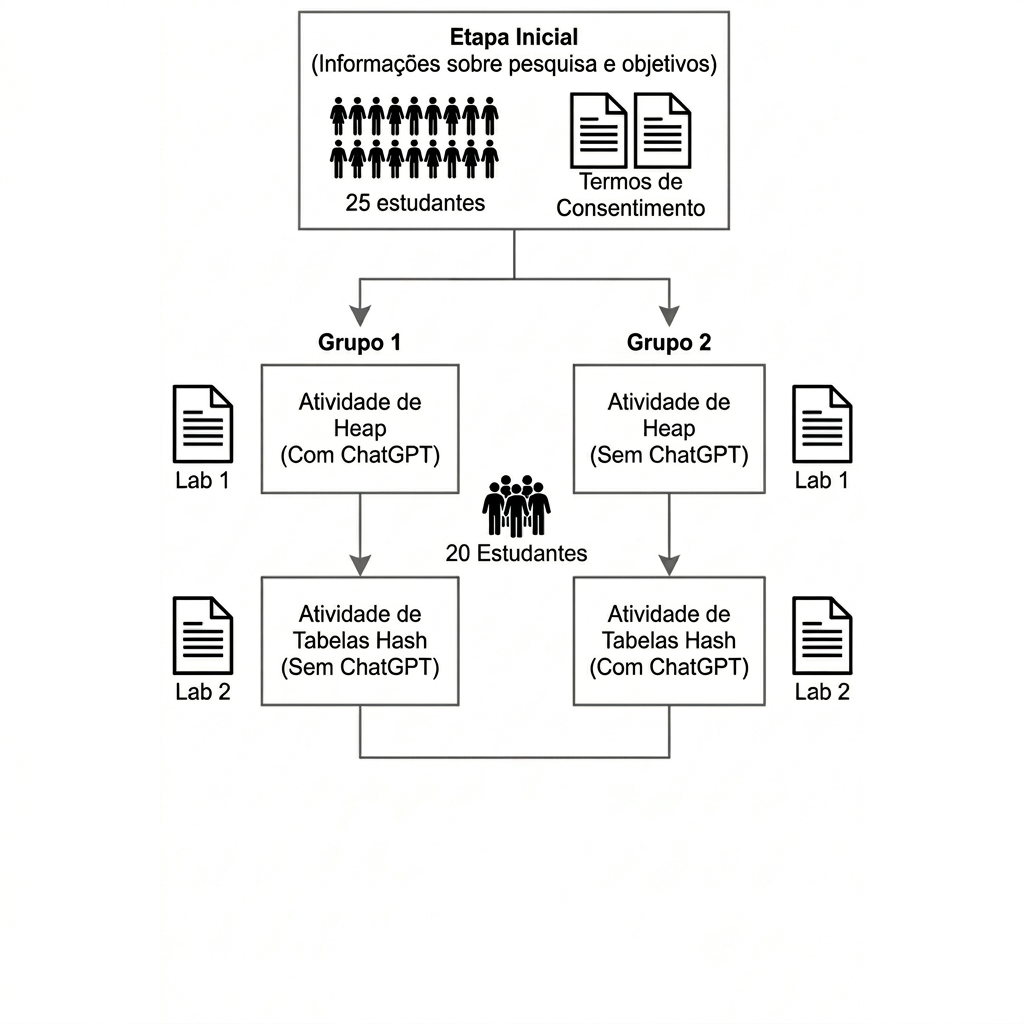
\includegraphics[width=\textwidth]{Figuras/fluxo-metodologia.png}
    \vspace{-0.4cm}
    \caption*{Fonte: Elaboração própria.}
    \label{fig:fluxo-metodologia}
\end{figure}

Na etapa inicial, os estudantes foram informados sobre a pesquisa, seus objetivos, as atividades previstas e as condições de participação. Antes do início das atividades experimentais, os participantes assinaram o termo de consentimento livre e esclarecido (TCLE) e responderam a perguntas sobre familiaridade prévia e frequência de uso de ferramentas de inteligência artificial generativa, especialmente em atividades de programação. Ao todo, 28 estudantes responderam a esse formulário, autorizando o uso dos dados exclusivamente para fins acadêmicos. A Tabela \ref{tab:perfil-ia} resume o perfil desses 28 respondentes quanto ao conhecimento e ao uso dessas ferramentas.

\begin{table}[!ht]
    \centering
    \caption{Perfil dos participantes quanto ao uso de IA generativa ($n = 28$, formulário inicial)}
    \label{tab:perfil-ia}
    \begin{tabular}{l c c}
        \hline
        \textbf{Indicador} & \textbf{$n$} & \textbf{Percentual} \\
        \hline
        Já conhecia IA generativa & 28 & 100,0\% \\
        \hline
        \multicolumn{3}{l}{\textit{Frequência de uso geral}} \\
        Mais de uma vez ao dia & 10 & 35,7\% \\
        Uma vez ao dia & 2 & 7,1\% \\
        Várias vezes na semana & 9 & 32,1\% \\
        Algumas vezes na semana & 7 & 25,0\% \\
        \hline
        \multicolumn{3}{l}{\textit{Uso em atividades de programação}} \\
        Sempre & 1 & 3,6\% \\
        Quase sempre & 25 & 89,3\% \\
        Raramente & 2 & 7,1\% \\
        \hline
    \end{tabular}

    \vspace{0.2cm}
    \caption*{Fonte: Elaboração própria, com base no termo de consentimento.}
\end{table}

Conforme a Tabela \ref{tab:perfil-ia}, todos os respondentes já possuíam conhecimento prévio sobre ferramentas de IA generativa e a maioria declarou utilizá-las com frequência em atividades de programação. Em seguida, os 25 participantes que integraram o experimento foram distribuídos aleatoriamente em dois grupos de tamanho semelhante --- Grupo 1 com 12 estudantes e Grupo 2 com 13 --- com condições invertidas de uso do ChatGPT:

\begin{itemize}
    \item \textbf{Grupo 1:} utilizou o ChatGPT na atividade prática de Heap e não utilizou a ferramenta na atividade prática de Tabelas Hash.
    \item \textbf{Grupo 2:} não utilizou o ChatGPT na atividade prática de Heap e utilizou a ferramenta na atividade prática de Tabelas Hash.
\end{itemize}

Esse arranjo, conhecido como desenho com grupos cruzados, permite que cada tópico seja estudado sob as duas condições experimentais, reduzindo o efeito de diferenças sistemáticas entre os conteúdos. Cada participante vivenciou uma atividade com a ferramenta e outra sem ela. A Tabela \ref{tab:resumo-participacao} resume a participação e as perdas amostrais ao longo do experimento.

\begin{table}[!ht]
    \centering
    \caption{Resumo da participação no experimento}
    \label{tab:resumo-participacao}
    \begin{tabular}{l c}
        \hline
        \textbf{Indicador} & \textbf{Quantidade} \\
        \hline
        Estudantes distribuídos nos grupos & 25 \\
        Participação completa (Heap e Tabelas Hash) & 20 \\
        Desistentes & 5 \\
        Grupo 1 com participação completa & 9 \\
        Grupo 2 com participação completa & 11 \\
        \hline
    \end{tabular}

    \vspace{0.2cm}
    \caption*{Fonte: Elaboração própria, com base na planilha de coleta do experimento.}
\end{table}

Dos 25 estudantes distribuídos, cinco não concluíram todas as etapas e foram excluídos da análise comparativa (três no Grupo 1 e duas no Grupo 2), resultando em 20 participantes com participação completa.

O experimento foi realizado em dois encontros distintos, cada um com duração aproximada de duas horas, abrangendo aula teórica, atividade prática e aplicação do questionário. No primeiro encontro, os participantes assistiram à aula teórica de Heap e, na sequência, realizaram a implementação prática em ambiente de laboratório e responderam ao questionário objetivo correspondente. As condições de uso do ChatGPT seguiram a divisão dos grupos descrita anteriormente. No grupo autorizado a usar a ferramenta, foi permitido o acesso à interface web do ChatGPT na versão gratuita, com seleção automática de modelo e uso livre, sem roteiro prévio de \textit{prompts}; no grupo sem ChatGPT, os estudantes puderam consultar materiais didáticos, anotações e documentação, mas não ferramentas de IA generativa. O docente e monitores acompanharam o laboratório para reforçar o cumprimento das condições. Ao término da atividade, todos responderam ao questionário sobre Heap, sem apoio do ChatGPT.

Aproximadamente 15 dias depois, ocorreu o segundo encontro, dedicado a Tabelas Hash, com a mesma estrutura (aula teórica, implementação prática e questionário), porém com as condições de uso do ChatGPT invertidas entre os grupos.

\section{Instrumentos e Materiais}
\label{sec:instrumentos-materiais}

As atividades práticas foram disponibilizadas por meio de repositórios que contêm código-base e métodos a serem implementados. Essa estrutura padronizou as tarefas e garantiu que todos os estudantes trabalhassem sobre os mesmos requisitos. O código-base continha apenas a estrutura necessária para orientar a implementação, sem fornecer diretamente a solução dos métodos avaliados.

O instrumento de avaliação foi composto por questionários objetivos de múltipla escolha (itens fechados). As questões foram selecionadas aleatoriamente a partir de bancos públicos de questões de entrevista técnica da plataforma Sanfoundry, alinhadas aos conteúdos de Heap e Tabelas Hash\footnote{Heapsort: \texttt{https://www.sanfoundry.com/heapsort-multiple-choice-questions-answers-mcqs/}. Hash tables (chaining): \texttt{https://www.sanfoundry.com/hash-tables-chaining-binary-trees-multiple-choice-questions-answers-mcqs/}.}. Cada acerto vale um ponto; a pontuação final de cada questionário é a soma dos acertos (0 a 20 em Heap; 0 a 21 em Tabelas Hash). Em ambos os casos, o uso do ChatGPT não foi permitido durante a aplicação do instrumento. Os questionários medem desempenho por reconhecimento e resposta a itens objetivos, e não pretendem capturar, por si sós, toda a profundidade da aprendizagem prática.

Os materiais do experimento, os enunciados das atividades, os instrumentos e os scripts de análise estatística estão disponíveis em repositório público no GitHub\footnote{\url{https://github.com/hellyaxs/MW-CL-pesquisa-tcc}}.

\section{Procedimentos de Coleta de Dados}
\label{sec:procedimentos-coleta}

A coleta de dados seguiu a sequência definida no desenho experimental. Inicialmente, os participantes receberam orientações sobre a pesquisa e foram distribuídos nos dois grupos. Em seguida, para o conteúdo de Heap, assistiram à aula teórica, realizaram a atividade prática sob a condição de uso do ChatGPT definida para seu grupo e responderam ao questionário correspondente, sem apoio da ferramenta.

Depois da conclusão dessa etapa, os estudantes participaram da aula teórica de Tabelas Hash, realizaram a atividade prática sob a condição invertida de uso do ChatGPT e responderam ao questionário sobre esse conteúdo, também sem apoio da ferramenta.

Os dados utilizados na análise comparativa foram as pontuações dos questionários de Heap e Tabelas Hash dos participantes com participação completa --- aqueles que cumpriram todas as etapas da pesquisa, desde o formulário de perfil até o último questionário. Foram excluídos da análise comparativa os cinco estudantes que não concluíram todas as etapas, embora parte deles tenha participado da etapa de Heap.

\section{Procedimentos de Análise dos Dados}
\label{sec:procedimentos-analise}

A análise dos dados foi organizada para avaliar a hipótese $H_{0}$. As pontuações de Heap e de Tabelas Hash foram reorganizadas por condição experimental --- com ChatGPT e sem ChatGPT --- e não por grupo de alocação inicial, conforme o desenho com grupos cruzados. A comparação inferencial principal considerou todas as pontuações de cada condição, totalizando 20 observações por condição na amostra completa. As pontuações foram analisadas na escala original de número de acertos, sem conversão para percentual ou outra normalização entre os questionários; essa diferença de escala (máximos 20 e 21) deve ser considerada na interpretação da comparação agregada.

Foram calculadas estatísticas descritivas das pontuações, incluindo média, mediana, desvio padrão, valores mínimo e máximo, tanto na comparação agregada entre condições quanto, de forma exploratória, separadas por conteúdo. Em seguida, verificou-se a distribuição dos dados por meio do teste de Shapiro--Wilk, como forma de avaliar a normalidade das pontuações em cada condição experimental.

Embora os resultados do teste de Shapiro--Wilk tenham indicado desvio significativo da normalidade em uma das condições, optou-se pela utilização do teste não paramétrico de Mann--Whitney U para a comparação agregada entre as pontuações com e sem uso do ChatGPT. Essa escolha foi motivada pelo tamanho reduzido da amostra, uma vez que testes não paramétricos tendem a apresentar maior robustez em estudos com número limitado de participantes \cite{kitchenham2019statistical,sheskin2003handbook}. A análise principal trata as pontuações reorganizadas por condição como duas amostras a serem comparadas quanto ao desempenho sob cada regime de uso da ferramenta. Reconhece-se, contudo, que o desenho com grupos cruzados produz, no nível do participante, um par de observações (uma com ChatGPT e outra sem); a opção pelo Mann--Whitney U agregado privilegiou a comparação entre condições na forma em que a hipótese $H_{0}$ foi formulada, em detrimento de um teste estritamente pareado, o que constitui uma limitação metodológica a ser considerada na interpretação dos resultados.

Os procedimentos descritivos e inferenciais foram executados em Python, com apoio da biblioteca SciPy para os testes de Shapiro--Wilk e de Mann--Whitney U, além do cálculo do Cliff's Delta implementado a partir das pontuações reorganizadas por condição.

Além da verificação da significância estatística, também foi calculado o coeficiente Cliff's Delta sobre a comparação agregada entre condições, com o objetivo de estimar a magnitude da diferença observada. Enquanto o teste de Mann--Whitney U permite verificar a existência de diferenças estatisticamente significativas, o Cliff's Delta complementa essa análise ao quantificar a intensidade do efeito encontrado. Para interpretação, adotaram-se os limiares propostos por Romano et al., conforme reportado por Kitchenham et al.: $| \delta | < 0{,}147$ indica efeito negligível; entre $0{,}147$ e $0{,}33$, pequeno; entre $0{,}33$ e $0{,}474$, médio; e acima de $0{,}474$, grande \cite{kitchenham2019statistical}.
